\section{Geometria de Uma e Duas Câmeras}

\subsection{Notação Básica de Geometria Projetiva}

Nesta seção, faremos uma breve introdução aos conceitos básicos de Geometria Projetiva e usaremos a notação contida em (citar hartley), por ser o tipo de notação mais difundido entre pesquisas de visão computacional. Para uma abordagem mais profunda do assunto o leitor pode pesquisar o referido autor.  

\subsubsection{O Espaço Projetivo em Duas Dimensões}



$\Longrightarrow$ A Reta


Sabemos que uma reta no plano $\mathbb{R}^{2}$ pode ser representada pela equação $a\,x+b\,y+c=0$, onde a reta fica perfeitamente determinada pelos valores das constantes $a,b,c$. Desta forma, podemos representar retas através de vetores, e assim a reta $a\,x+b\,y+c=0$ seria representada por $(a,b,c)^T \in \mathbb{R}^{3}$, utlizando o símbolo em negrito $\lightrgb$ para indicar tal vetor escrito em coluna, por padrão. Portanto $\lightrgb = (a,b,c)^T$. Note que a relação entre uma dada reta e o seu respectivo vetor não é biunívoca, pois o vetor $k\,(a,b,c)^T$, tal que $k \in \mathbb{R}$, representa a reta $k\,a\,x+k\,b\,y+k\,c=0$ que é a mesma reta $a\,x+b\,y+c=0$. Temos, então, infinitos vetores (chamados paralelos na Álgebra Linear) que representam uma mesma reta e formam uma classe de equivalência, onde essa classe pode ser repsentada por qualquer um de seus vetores. Os vetores de uma classe de equivalência, definida pela multiplicação por um escalar, são conhecidos como vetores {\it homogêneos}. O conjunto de classes de equivalência de vetores em $\mathbb{R}^{3} - (0,0,0)^T$ forma o {\it Espaço Projetivo} $\mathbb{P}^{2}$. O vetor $(0,0,0)^T$ foi excluído por não representar reta alguma. Após essas considerações, dizemos que uma reta no plano é representada pelo vetor $(a,b,c)^T$ em {\it coordenadas homogêneas}. Já que para determinar um reta precisamos determinar os valores do três parâmetros $a,b \text{e} c$, vemos que uma reta tem três graus de liberdade.

$\Longrightarrow$ O Ponto


Sabemos também, que em $\mathbb{R}^{2}$ os pontos são representados através de pares ordenados do tipo $(x,y)$, assim cada ponto pode ser identificado como um vetor $(x,y)^T$. Os vetores que se referem a pontos serão representados pelo símbolo em negrito $\x$, que sempre indicará um vetor coluna. Desse jeito, $\x=(x,y)^T$. Sabemos também que um ponto $(x,y)^T$ pertence a uma reta $(a,b,c)^T$ se, e somente se $a\,x+b\,y+c=0$, e podemos realizar essa verificação utilizando multiplicação matricial, escrevendo $\x$ com uma terceira coordenada igual a 1:

\begin{center}
$\begin{array}{ccccc}
 (x,y,1)^T 
&\begin{pmatrix}
 a  \\ 
 b  \\ 
 c 
 \end{pmatrix} 
& = 0 \qquad 
& \text{ou} 
& \qquad \x ^T\lightrgb = 0.
\end{array}$
\end{center}

Ou seja, temos um ponto de $\mathbb{R}^{2}$ representado como um vetor com três coordenadas. Observe que para $k \in \mathbb{R} - \{0\}$, temos:

\begin{center}
$\begin{array}{ccccccc}
 (k\,x,k\,y,k)^T 
&\begin{pmatrix}
 a  \\ 
 b  \\ 
 c 
 \end{pmatrix} 
& = 0
& \qquad \leftrightarrow \qquad
& (x,y,1)^T
&\begin{pmatrix}
 a  \\ 
 b  \\ 
 c 
 \end{pmatrix} 
& = 0.
\end{array}$
\end{center}

Portanto,  variando $k$, podemos considerar os vetores em coordenadas homogeneas $(k\,x,k\,y,k)^T \in \mathbb{P}^2$, como representantes do mesmo ponto $(x,y)^T \in \mathbb{R}^2$, e podemos resgatar nossa representaçao original aplicando o procedimento $(x/k,y/k)^T$, pois $k \ne 0$.

\begin{figure}[!htb]
\centering
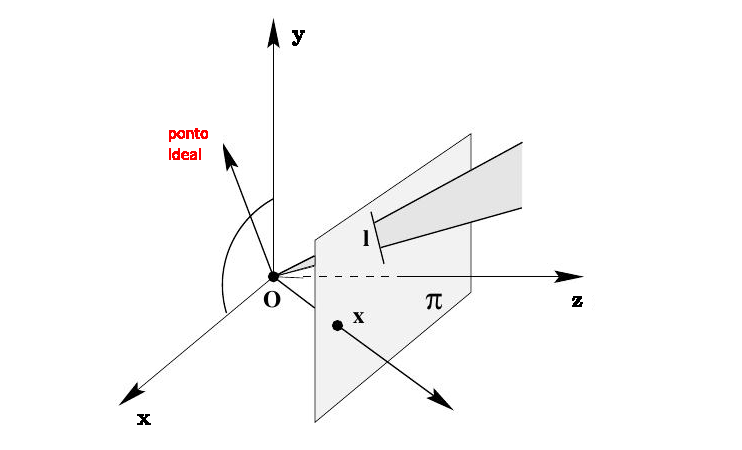
\includegraphics[scale=0.8]{espaco_P2}
\caption{O plano $\pi$ representa o espaço projetivo $\mathbb{P}^2$. Pontos e retas pertencentes a esse espaço são representados, respectivamente, por raios e planos que passam pela origem do $\mathbb{R}^3$.}
\label{plano_P2}
\end{figure}

Podemos pensar no esapaço projetivo como um conjunto de raios passando pela origem do $\mathbb{R}^3$, onde cada raio representa um único ponto, que é a interseção desse raio com o plano $\mathbb{P}^2$. Desta mesma forma, retas em $\mathbb{P}^2$ são formadas por planos. Na figura \ref{plano_P2}, podemos observar como a interseção do raio com o plano define um ponto, assim como a interseção de dois planos definem uma reta.


Para determinar um ponto precisamos determinar os valores das duas primeiras coordenadas do vetor homogêneo que representa esse ponto, já que a terceira coordenada está em função das duas primeiras. Assim, dizemos que um ponto tem dois graus de liberdade e a terceira coordenada pode ser usada para fixar uma escala.
\\

$\Longrightarrow$ A Cônica


Em geometria Euclidiana, as cônicas são de três tipos principais: elipse, hipérbole e parábola. São definidas, algebricamente, por uma equação do segundo grau em duas variáveis, considerando coordenadas não homogêneas:

\begin{equation*}
a\,x^2+b\,x\,y+c\,y^2+d\,x+e\,y+f=0.
\end{equation*}

Sabemos que um ponto pertence à cônica se ele é solução da equação acima, a qual pode ser representada utilizando multiplicação matricial e vetores em coordenadas homogêneas, com a terceira coordenada configurada como 1:

\begin{center}
$
\begin{array}{cccc}
  (x,y,1)^T 
& \begin{bmatrix}
a & b/2 & d/2\\
b/2 & c & e/2\\
d/2 & e/2 & f
\end{bmatrix}
& \begin{pmatrix}
x\\
y\\
1
\end{pmatrix}
& = 0.
\end{array}
$
\end{center}

Podemos generalizar essas coordenadas homogêneas fazendo as substituições $x = x_{1}/x_{3}$ e $y = x_{2}/x_{3}$, e nossa equação do elípse fica:

\begin{equation*}
a\,x_1^2+b\,x_1\,x_2+c\,x_2^2+d\,x_1\,x_3+e\,x_2\,x_3+f\,x_3^2=0.
\end{equation*}

Novamente em notação matricial:

\begin{center}
$
\begin{array}{cccccc}
  (x_1,x_2,x_3)^T 
& \begin{bmatrix}
  a & b/2 & d/2\\
  b/2 & c & e/2\\
  d/2 & e/2 & f
  \end{bmatrix}
& \begin{pmatrix}
  x_1\\
  x_2\\
  x_3
  \end{pmatrix}
& = 0
& \qquad \text{ou} \qquad
& \x^T\,C\,\x = 0.
\end{array}
$
\end{center}

Já que um ponto pertence à cônica se, e somente se, satisfaz a última equação, temos que $C$ fica definida como a matriz que representa uma cônica no espaço projetivo $\mathbb{P}^2$.

\begin{center}
$
\begin{array}{cc}
C = & \begin{bmatrix}
      a & b/2 & d/2\\
      b/2 & c & e/2\\
      d/2 & e/2 & f
      \end{bmatrix}.
\end{array}
$
\end{center}


Percebemos que as cônicas são representadas por matrizes $3\times3$ simétricas e, portanto, possuem seis variáveis. Usando uma dessas variáveis para fixar a escala, temos que as cônicas possuem cinco graus de liberdade. Podemos, por exemplo, dividir todas as coordenadas da matriz $C$ por $f$. 

\subsubsection{O Espaço Projetivo em Três Dimensões}


$\Longrightarrow$ O Ponto


Analogamente à representação de um ponto no espaço $\mathbb{P}^2$, um ponto no espaço $\mathbb{P}^3$ é repesentado através de coordenadas homogêneas, acrescentando-se uma quarta coordenada ao vetor que representa esse ponto. Desta forma, $\X = (X_1,X_2,X_3,X_4)^T$ e $X_4 \ne 0$, onde $\X$ é a representação em coordenadas homogêneas do ponto $(X,Y,Z)^T \in \mathbb{R}^3$. Portanto esse vetor continua tendo três graus de liberdade. Para realizar tal mudança basta tomar 

\begin{equation*}
X=X_1/X_4 \,\, ,\, Y=X_2/X_4 \,\,\, \text{e} \,\,\, Z=X_3/X_4.
\end{equation*}

 


$\Longrightarrow$ O Plano

Temos que a representação algébrica de um plano $\bpi$ no espaço $\mathbb{R}^3$ é dada pela equação

\begin{equation*}
\pi_1\,X+\pi_2\,Y+\pi_3\,Z+\pi_4=0.
\end{equation*}

Um ponto pertence ao plano se, e somente se, satifaz a equação acima que na forma matricial usando a representação do ponto em coordenadas homogêneas fica:

\begin{center}
$
\begin{array}{ccc}
  (\pi_1,\pi_2,\pi_3,\pi_4)^T
& \begin{pmatrix}
  X\\
  Y\\
  Z\\
  1
  \end{pmatrix}
& = 0.
\end{array}
$
\end{center}

Fazendo as substituições 
\begin{equation*}
X=X_1/X_4 \,\, , \,\, Y=X_2/X_4 \,\,\,\, \text{e} \,\,\,\, Z=X_3/X_4 ,
\end{equation*}

generalizamos a representação do ponto e a equação se torna:

\begin{center}
$
\begin{array}{ccccc}
(\pi_1,\pi_2,\pi_3,\pi_4)^T
& \begin{pmatrix}
  X_1\\
  X_2\\
  X_3\\
  X_4
  \end{pmatrix}
& = 0
& \qquad \text{ou} \qquad
& \bpi^T \,\, \X = 0.
\end{array}
$
\end{center}


Desta forma, verificamos que, assim como os pontos, um plano $\bpi = (\pi_1,\pi_2,\pi_3,\pi_4)^T$ fica inteiramente determinado por um vetor com quatro coordenadas em $\mathbb{P}^3$. Aqui temos uma analogia com o espaço $\mathbb{P}^2$, já que pontos e retas têm a mesma representação vetorial com três coordenadas naquele espaço. Como multiplicar a equação algébrica de um plano por um escalar diferente de zero não altera seu valor, temos que os planos possuem três graus de liberdade. Podemos dividir as três primeiras coordenadas pela última, por exemplo, e fixar um escala.

Obs: As três primeiras coordenadas do vetor que representa o plano corresponde ao vetor normal ao plano, conforme definido em Álgebra Linear.
\\


$\Longrightarrow$ A Reta

Uma reta pode ser definida passando por dois pontos. Em $\mathbb{P}^2$, como os dois pontos estão no mesmo plano, uma reta passando por esses dois pontos tem apenas três graus de liberdade, conforme visto anteriormente. Mas em $\mathbb{P}^3$, como os dois pontos podem estar em planos diferentes, temos que uma reta apresenta quatro graus de liberdade, dois graus para cada ponto. Assim, uma reta deveria ser representada por um vetor com cinco coordenadas em $\mathbb{P}^3$, mas vetores desse tipo não podem ser usados, facilmente, em expressões matemáticas que envolvem vetores com quatro coordenadas representando pontos e planos. Portanto é necessário encontrar uma outra representação, e uma das formas mais simples é definir a reta através de dois pontos não coincidentes.


Uma reta ${\bf L}$ passando por dois pontos ${\bf A} \,\,\, \text{e} \,\,\, {\bf B}$ é representada pelo espaço linha gerado pela matriz $W$ composta pelos pontos ${\bf A}^T \,\,\,\text{e} \,\,\, {\bf B}^T$ em linha:

\begin{center}
$
\begin{array}{cc}
W = 
& \begin{bmatrix}
  A^T\\
  B^T
  \end{bmatrix},
\end{array}
$
\end{center}
onde os espaço gerado por $W^T$ é o conjunto de pontos do tipo $a\,{\bf A} + b\,{\bf B}$ pertencentes à reta ${\bf L}$ procurada. Outras representações de uma reta no espaço projetivo $\mathbb{P}^3$ podem ser encontradas em (citar hartley).


$\Longrightarrow$ A Quádrica


Similarmente à cônica em $\mathbb{P}^2$, uma quádrica $Q$ em $\mathbb{P}^3$ é definida pela equação

\begin{equation*}
\X^T\,Q\,\X = 0,
\end{equation*}
onde $Q$ é uma matriz simétrica $4\times4$ com nove graus de liberdade.




\begin{figure}[!htb]
$
\begin{array}{cc}
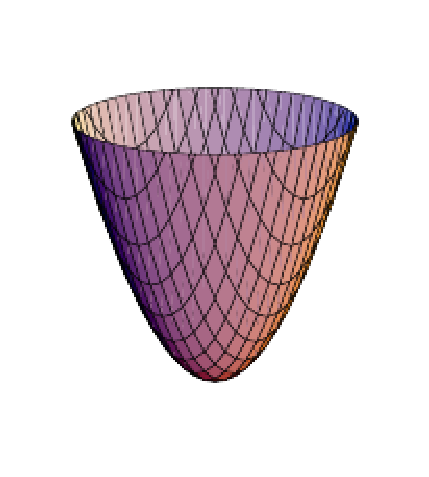
\includegraphics[scale=1.1]{paraboloide}
&
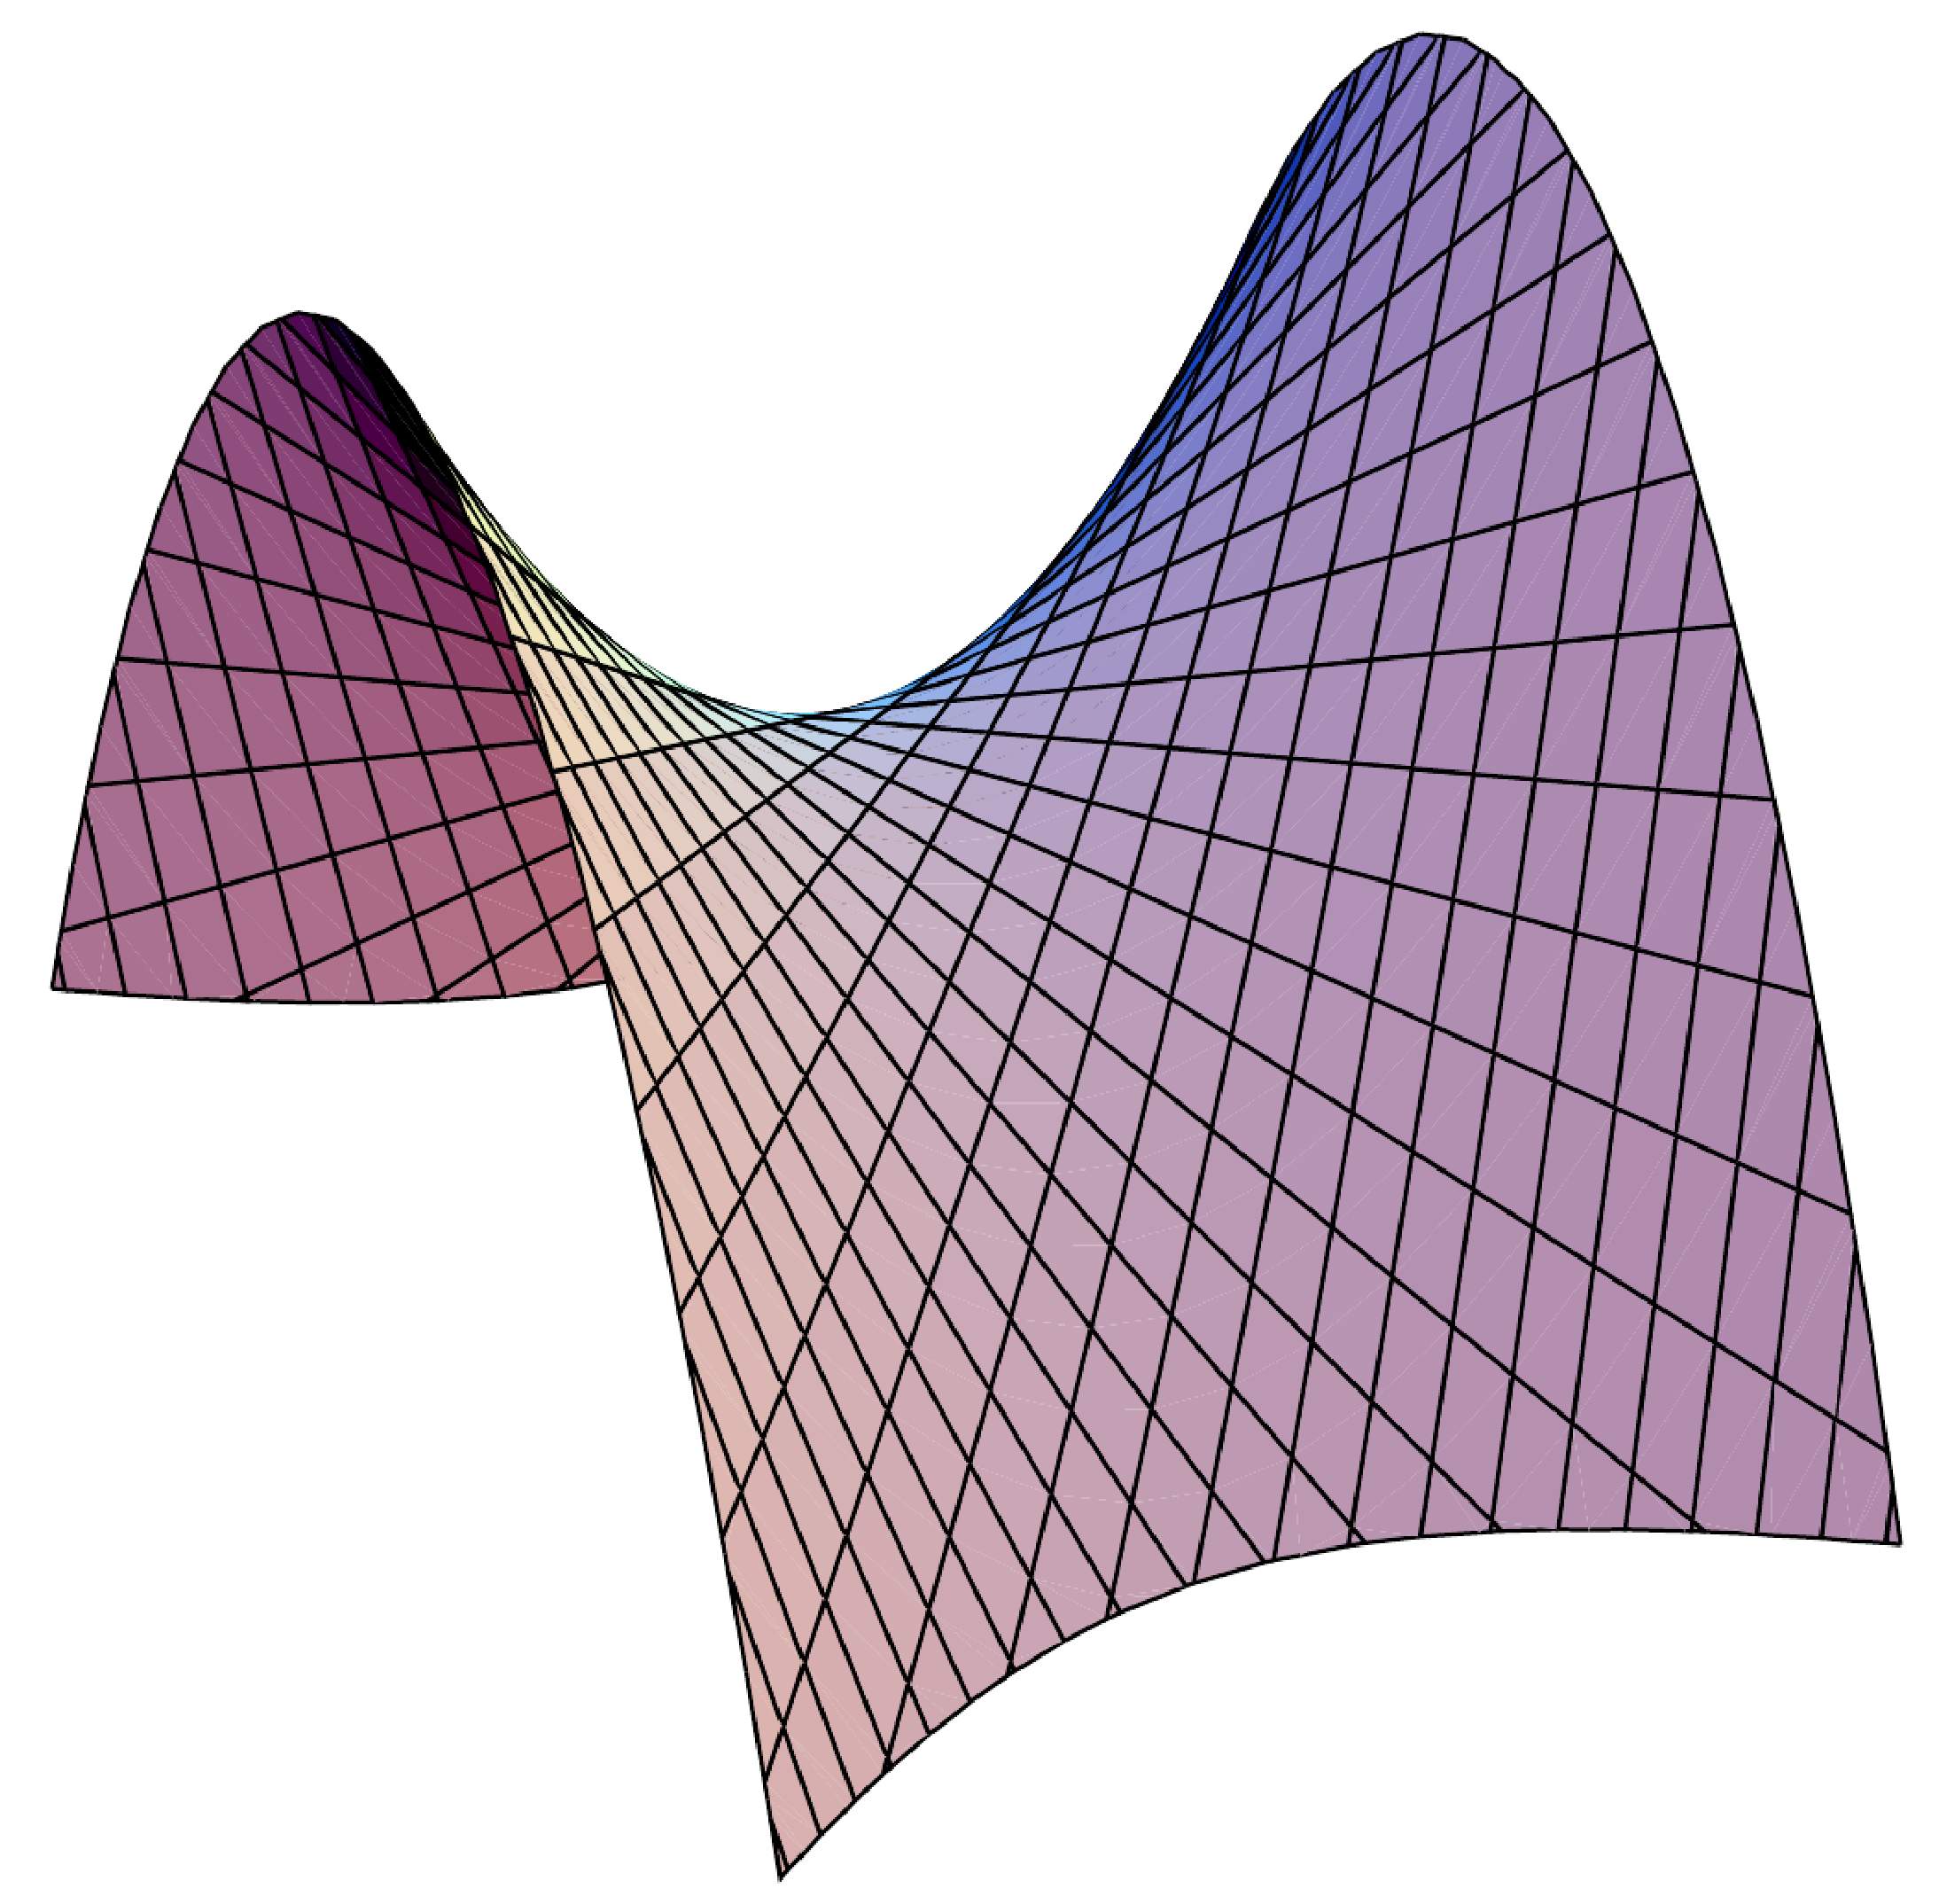
\includegraphics[scale=0.9]{hiperboloide_1_folha}
\end{array}
$
\caption{Parabolóide à esquerda e hiperbolóide de uma folha à direita.}
\label{quadricas}
\end{figure}


Podemos observar na figura \ref{quadricas} dois exemplos de quádricas.

\subsubsection{A Câmera P}

A câmera é uma transformação linear entre um ponto 3D no espaço e um ponto 2D no plano da imagem, representada por uma matriz com algumas propriedades que realizam o mapeamento entre os pontos. Existem varios tipos de camera, mas para tratar das caracteristicas basicas vamos utilizar o modelo buraco de alfinete, do ingles \textit{pinhole}.

Consideramos o centro de projeçao, ou centro da camera, como a origem do espaço tridimensional Euclidiano, com o plano da imagem ou plano focal sendo $Z = f$, onde $f$ e a distancia focal entre o plano da imagem e o centro de prjeçao. Como podemos obeservar na figura \ref{camera}, um ponto no espaço $\X$  mapeado a um ponto $\x$ no plano da imagem por uma reta que liga $\X$ ao centro de projeção e intersepta o plano da imagem. Assim, ignorando a última coordenada, temos o mapeamento:

\begin{center}
$\X = (X,Y,Z)^T \rightarrow \x = (fX/Z,fY/Z,f) \rightarrow (fX/Z,fY/Z)$  
\end{center}

O plano que passa pelo centro da câmera e é paralelo ao plano da imagem é chamado plano principal, é o plano $xy$ na figura \ref{camera}. O eixo principal passa pelo centro da câmera e é perpendicular ao plano da imagem, onde a interseção desse eixo com o plano da imagem forma o ponto principal.


\begin{figure}[!htb]
\centering
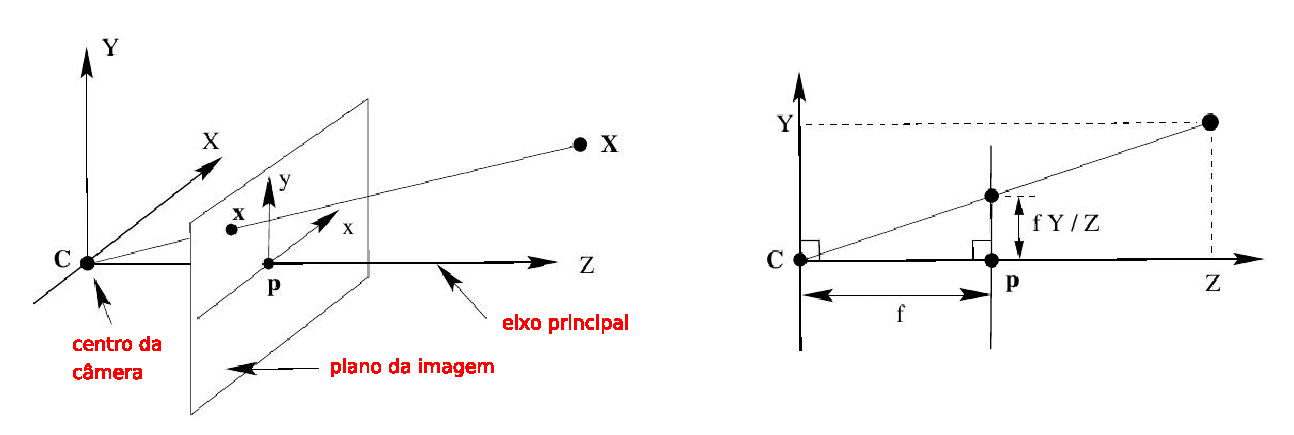
\includegraphics[scale=.64]{modelo_camera}
\caption{Visualização das características básicas de uma câmera como distância focal, eixo principal, plano da imagem e centro de projeção.}
\label{camera}
\end{figure}

Com vetores representados em coordenadas homogêneas, podemos expressar no mapeamento através de um operador linear, onde realizamos a multiplicação da matriz $P$ que representa a câmera  por um ponto no espaço, resultando num ponto na imagem conforme o esquema abaixo:

\begin{center}
$
\begin{array}{ccc}
\begin{pmatrix}
fX\\
fY\\
Z
\end{pmatrix} = 
&
\begin{bmatrix}
f& & &0\\
 &f& &0\\
 & &1&0
\end{bmatrix}
&
\begin{pmatrix}
X\\
Y\\
Z\\
1
\end{pmatrix}
\end{array}
$
\end{center}


\subsection{Notação Usada por Fabbri}
Usar figura do artigo.

\subsection{Resumo dos Resultados Fabbri}
Projeção e reconstrução 3D com o uso de tangentes.
